\documentclass[smaller,spanish,xcolor=svgnames]{beamer}

% Paquetes personalizados
\usepackage{paquetes} 
\usepackage{colores}
\usepackage{modo}
\usepackage{licencia}
% -------------------------------------------------------------------

\title[Sistemas Expertos]{{\Huge Sistemas Expertos} \\ Diseño de Videojuegos}

\author[Manuel Palomo Duarte - José Tomás Tocino]{Manuel Palomo Duarte \\ José Tomás Tocino García}

\date{Junio de 2011}

\begin{document}

\begin{frame}
  \titlepage
\end{frame}

\section{Definiciones}
\subsection{¿Qué es un sistema experto?}
\begin{frame}{¿Qué es un sistema experto?}
    \begin{itemize}
    \item \textbf{Sistema experto:} mecanismo que \textbf{simula} el
      conocimiento de un experto humano en una materia determinada.
    \item Se usan con éxito en muchas ramas de la ciencia: medicina, ingeniería, etc.
    \item Existen varios tipos:
      \begin{itemize}
      \item Basados en \textbf{reglas}. Son los que estudiaremos.
      \item Basados en \textbf{casos}.
      \item Basados en \textbf{redes bayesianas}.
      \end{itemize}
    \end{itemize}
\end{frame}

\subsection{Componentes de un SEBR}
\subsubsection{Componentes principales}

\begin{frame}{Componentes principales}
  \begin{block}{Hechos}
    Información sobre el entorno que el sistema lee y utiliza para tomar
    decisiones.
  \end{block}

  \begin{block}{Reglas}
    Condiciones que el sistema evalúa a partir de los hechos presentes para
    generar nuevo conocimiento.
  \end{block}

  \begin{block}{Motor de inferencia}
    Se encarga de decidir qué reglas pueden activarse según los hechos presentes.
  \end{block}
  
\end{frame}

\subsubsection{Componentes secundarios}

\begin{frame}{Componentes secundarios}
    \begin{block}{Lista de activación (del inglés \textit{agenda})}
      Contiene las reglas cuyas condiciones se han cumplido y son candidatas a
      dispararse.
    \end{block}

    \begin{block}{Estrategias de resolución de conflictos}
      Habrá ocasiones en las que varias reglas podrán ser candidatas, hay que
      decidir qué reglas disparar en cada caso.
    \end{block}
  
\end{frame}

\section{CLIPS}

\section{Gades Siege}


% \section{Análisis Léxico}
% \begin{frame}{Tokens definidos}
%   \begin{columns}[c]
%     \begin{column}{0.5\hsize}
%       \begin{itemize}
%       \item \textbf{CHAR}
%       \item \textbf{INT}
%       \item \textbf{FLOAT}
%       \item \textbf{VOID}
%       \item \textbf{LITERAL\_STRING}
%       \item \textbf{LITERAL\_CHAR}
%       \item \textbf{LITERAL\_INT}
%       \item \textbf{LITERAL\_FLOAT}
%       \end{itemize}
%     \end{column}
%     \begin{column}{0.5\hsize}
%       \begin{itemize}
%       \item \textbf{IF}
%       \item \textbf{ELSE}
%       \item \textbf{RETURN}
%       \item \textbf{ID}
%       \item '+', '-', '*', '/', '='
%       \item '[', ']', '(', ')', '\{', '\}'
%       \item ';', '\&'
%       \end{itemize}
%     \end{column}
%   \end{columns}
% \end{frame}

% \section{Análisis Sintáctico}

% \begin{frame}{Gramática diseñada}
%   \begin{block}{Criterios seguidos}
%     \begin{itemize}
%     \item Sencillez
%     \item Posible ampliación del subconjunto de C soportado
%     \item Acciones semánticas para depurar el analizador
%     \end{itemize}
%   \end{block}
%   \begin{block}{Problemas encontrados}
%     \begin{itemize}
%     \item Algunas restricciones ``ensucian'' la gramática
%     \item ¿Dónde especificamos los punto y coma?
%       \begin{itemize}
%       \item Al final de una \textbf{declaración}
%       \item Al final de una \textbf{sentencia que es una expresión}
%       \item Al final de una \textbf{sentencia return}
%       \end{itemize}
%     \end{itemize}
%   \end{block}
% \end{frame}

% \begin{frame}{Construcción del ASA}
%   Diagrama de clases de los nodos implementados:
%   \begin{center}
%     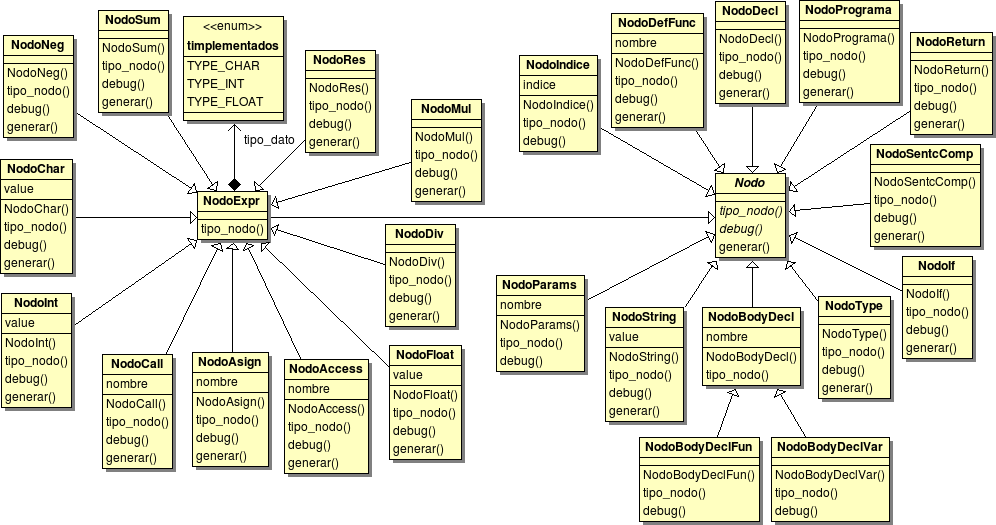
\includegraphics[width=\textwidth]{./img/nodos.png}
%   \end{center}
% \end{frame}

% \begin{frame}{Construcción del ASA}
%   Para crear el ASA iremos creando y enlazando los nodos a través de
%   las acciones semánticas.
%   \begin{block}{El \textbf{gran} problema}
%     \begin{itemize}
%     \item Programar las acciones semánticas para crear el ASA es una
%       tarea \textbf{repetitiva} propensa a errores
%     \item Toda la posterior \textbf{generación de código} se basará en
%       la corrección del ASA
%     \end{itemize}
%   \end{block}
%   \pause
%   \begin{alertblock}{La \textbf{gran} pregunta}
%     \begin{center}
%       ¿Cómo podemos \textbf{comprobar} el ASA generado?
%     \end{center}
%   \end{alertblock}
%   \pause

% \begingroup
% \setbeamercolor{block title}{bg=verde2}
% %\setbeamercolor{block body}{bg=yellow,fg=verde2}%
%   \begin{block}{La \textbf{gran} respuesta}
%     \begin{center}
%       \textbf{GraphViz}
%     \end{center}
%   \end{block}
% \endgroup
% \end{frame}

% \begin{frame}{Dibujado del ASA con GraphViz}
%   Definición de la función factorial
%   \lstinputlisting{../proyecto/test/factorial.c}
%   \begin{center}
%     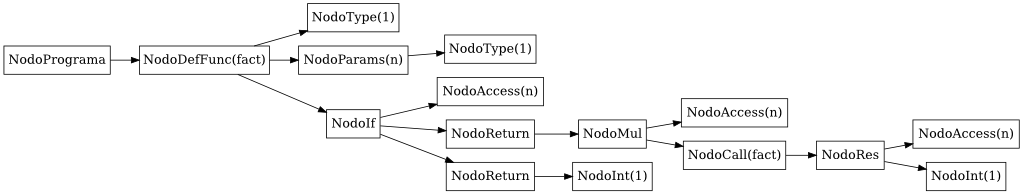
\includegraphics[width=\textwidth]{./img/grafo.png}
%   \end{center}
% \end{frame}

% \begin{frame}{Generación de código ensamblador IA32}
%   Una vez depurado el código para la generación del ASA, ya estamos en
%   disposición de generar código ensamblador para IA32.
%   \begin{block}{Dificultades}
%     Generar \textbf{código ensamblador para IA32} es mucho más
%     \textbf{difícil} que generar \textbf{código para GraphViz}, la dos
%     razones principales son:
%     \begin{itemize}
%     \item Declaraciones
%     \item Tipos
%     \end{itemize}
%   \end{block}
%   \pause

%   \begingroup
%   \setbeamercolor{block title}{bg=verde2}
%   \begin{block}{La solución}
%     \begin{center}
%       Tabla de Símbolos
%     \end{center}
%   \end{block}
%   \endgroup

% \end{frame}

% \begin{frame}{Tabla de símbolos con ámbitos anidados}
%   Estructura auxiliar que nos permita almacenar información durante el
%   proceso de compilación.
%   \begin{center}
%     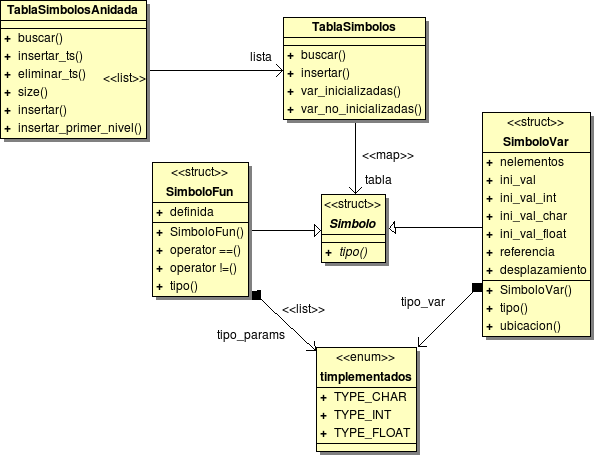
\includegraphics[width=8cm]{./img/tabla.png}
%   \end{center}
% \end{frame}

% \begin{frame}{Tabla de símbolos con ámbitos anidados}
%   Relación entre la tabla de símbolos y los ámbitos:
%   \pause
%   \begin{block}{Declaraciones globales}
%     Tendremos una \textbf{TablaSimbolos} global al programa.
%   \end{block}
%   \pause
%   \begin{block}{Definición de funciones}
%     Crearemos una \textbf{TablaSimbolosAnidada}, el cuya primera
%     posición copiaremos la \textbf{TablaSimbolos} global.
%   \end{block}
%   \pause
%   \begin{block}{Nuevos ámbitos}
%     Cada nuevo ámbito dentro de la definición de una función supondrá
%     añadir una nueva \textbf{TablaSimbolos} en tope de la pila de la
%     \textbf{TablaSimbolosAnidada} asociada a la función.
%   \end{block}
% \end{frame}

% \begin{frame}{Inferencia, Chequeo y Conversión de tipos}
%   La inferencia, chequeo y conversión de tipos están asociados a los
%   \textbf{NodosExpr}.
%   \begin{block}{Inferencia de tipo}
%     \begin{itemize}
%     \item \textbf{NodoInt, NodoChar, NodoFloat:} De forma inmediata
%     \item \textbf{NodoNeg:} Genera el mismo tipo de entrada
%     \item \textbf{NodoAccess:} Su tipo viene de la tabla de símbolos
%     \item \textbf{NodoSum, NodoRes, NodoMul, NodoDiv:} Genera el tipo
%       más general de sus operandos
%     \item \textbf{NodoAsign:} Genera siempre el tipo de la variable
%       donde se asigna el valor
%     \item \textbf{NodoCall:} Genera siempre el tipo declarado como
%       salida
%     \end{itemize}
%   \end{block}
% \end{frame}

% \begin{frame}{Inferencia, Chequeo y Conversión de tipos}
%   El chequeo y conversión se producen en aquellas expresiones que
%   tienen declaraciones de tipo asociadas.
%   \begin{block}{NodoAsign}
%     La expresión asignada se trata de convertir al tipo de la
%     variable, en caso de que no sea posible devolveremos un error.
%   \end{block}
%   \pause
%   \begin{block}{NodoCall}
%     Los argumentos que recibe son convertidos al tipo declarado, en
%     caso de que no fuera posible daremos un error.
%   \end{block}
%   \pause
%   \begin{block}{Operaciones Binarias: NodoSuma, NodoResta, ...}
%     Los argumentos que recibe A y B son convertidos al tipo más general
%     de ambos.
%   \end{block}
% \end{frame}

% \begin{frame}{Flotantes y Cadenas literales}
%   En la arquitectura IA32, estos dos tipos no son manejados
%   directamente, sino que se usa las direcciones de memoria que los
%   contienen.
%   \begin{block}{Tratamiento de Flotantes y Cadenas literales}
%     \begin{itemize}
%     \item Definiremos dos diccionarios <valor, dirección>
%       \pause
%     \item Cuando nos encontramos un nuevo valor, creamos una nueva
%       entrada en el diccionario asignándole una dirección.
%       \pause
%     \item Cuando nos encontramos con valor aparecido anteriormente le
%       asignamos a éste la dirección declarada previamente.
%       \pause
%     \item Al final debemos declarar en el código ensamblador todos lo
%       valores en las direcciones pertinentes según el diccionario.
%     \end{itemize}
%   \end{block}
% \end{frame}

% \section{Fin}

% \begin{frame}{Para terminar...}
%   \begin{center}
%     \Huge \textcolor{verde2}{Demostración}\\

%     \vspace*{1cm}
    
%      \Large ¿Preguntas?
%   \end{center}
% \end{frame}



\end{document}







